%!TEX TS-program = lualatex
%!TEX encoding = UTF-8 Unicode
%% (this document must be compiled with LuaLaTeX) 
%% Main file for PFPE gravimeter documentation
%% 
%% Formatting loosely based on the Overleaf Software Manual and Technical Document Template	
%% 									

\documentclass{pfpe-manual}

% Packages used in this example
\usepackage{graphicx}  % for including images
\usepackage{microtype} % for typographical enhancements
\usepackage[letterpaper,top=4.2cm,bottom=4.2cm,left=3.5cm,right=3.5cm]{geometry} % for setting page size and margins

% Custom macros used in this example document
\newcommand{\doclink}[2]{\href{#1}{#2}\footnote{\url{#1}}}
%\newcommand{\cs}[1]{\texttt{\textbackslash #1}}

% Frontmatter data; appears on title page
\title{gravitron manual}
\version{1.0.0}
\author{Hannah F. Mark}
\license{CC-BY 4.0}
%%%%%%%%%%%%%%%%%\softwarelogo{\includegraphics[width=8cm]{figs/grav_photo}}

\begin{document}

\maketitle

\tableofcontents
\newpage

\section{Introduction}

gravitron is a GUI software tool for recording gravity ties and calculating meter biases. It is designed for the Potential Fields Pool Equipment (PFPE) DGS gravimeters used onboard UNOLS vessels.

\section{Installation}
\label{install}
gravitron is an electron app written in javascript. If you read that last sentence and thought ``ok, I know what to do with that'' then feel free to grab the source code (\url{https://github.com/hfmark/gravitron}), and compile and run as you would any similar program on your operating system of choice. If you're not as used to programs like this, read on for some instructions.

\subsection{Linux and Mac OS}
\label{inst:unix}
%\paragraph{Option 1: pre-compiled binaries}
%Pre-compiled binaries for the latest Ubuntu LTS release (22.04) and for Mac OSX (currently, 12) are available on github. Navigate to \url{https://github.com/hfmark/gravitron/releases} and download the zip archive for your operating system. Make a folder where you want to keep all of the program files, and unzip all of the contents of the archive into that folder.
%
%If you are on Mac OSX, you will also (probably) need to install the GNU C compilers and GTK3, since the binary you downloaded from github is compiled against libraries that will not otherwise be on your computer. I recommend using \href{https://brew.sh/}{homebrew} for this. Once you have homebrew set up, run the following commands in a terminal:
%\begin{verbatim}
%brew install gcc
%brew install gtk+3
%\end{verbatim}
%This should (hopefully) enable you to run the pre-compiled binary.
%
%\paragraph{Option 2: build from source}
%The source code for gravitron is available on github at \url{https://github.com/hfmark/gravitron/releases}. Download and unzip the archive, which includes all auxiliary files and a Makefile for building the program.
%
%In order to compile the program, you will need the GNU C compiler(s) and the GTK3 library. To compile using the provided Makefile, you will also need the \texttt{make} tool and \texttt{pkg-config}. To install all of the necessary things in Ubuntu, run the following commands in a terminal:
%\begin{verbatim}
%sudo apt install gcc g++ make pkg-config
%sudo apt install libgtk-3-dev
%\end{verbatim}
%
%To install those same things in Mac OSX, I recommend using \href{https://brew.sh/}{homebrew}. Once you have homebrew set up per their instructions, prepare to install gravitron by running the following commands in a terminal:
%\begin{verbatim}
%brew install gcc
%brew install pkg-config
%brew install make
%brew install gtk+3
%\end{verbatim}
%If you have Xcode and the Xcode developer tools installed you may already have some of the prerequisites installed, but adding the brew versions shouldn't hurt anything.
%
%Next, open a terminal and navigate to the folder where you put all of the source files you got from github. For example, if I had put the files in a folder called `gravties' that was on my desktop, I could enter 
%\begin{verbatim}
%cd ~/Desktop/gravties
%\end{verbatim}
%in the terminal to move to that location in the file system. You can also right click on the folder in the file browser and select ``Open in terminal.'' Then, to build the program, simply enter the command
%\begin{verbatim}
%make
%\end{verbatim}
%
%If you are running a linux distro other than Ubuntu, it's likely that you know enough about the system to figure out how to adapt those commands to your needs. If not, see Section~\ref{helphelp} for suggestions on where to go for help.

\subsection{Windows}
\label{inst:wind}
%Windows is a little less friendly to this kind of program than unix-based systems, so there are a few more steps to go through, but in the end it should still work just fine. 
%
%First, we will use MSYS2 to set up a unix-friendly environment to run the program. Download the installer from \href{https://www.msys2.org/}{the MSYS2 website} and run it, accepting all the default settings for installation. When the installer finishes, select the ``Run MSYS2 now'' option, and a UCRT64 terminal will open. Right click on the title bar of that terminal window and select ``Pin to taskbar'' to make this particular terminal environment easier to find later (if you don't pin it, you can re-open the UCRT64 terminal from the file browser using This PC -> Local Disk (C:) -> msys64 -> ucrt64.exe).
%
%Now, in your UCRT64 terminal, run the following commands to install the libraries for gravitron:
%\begin{verbatim}
%pacman -S mingw-w64-ucrt-x86_64-gcc
%pacman -S mingw-w64-ucrt-x86_64-gtk3
%\end{verbatim}
%For each of those commands, when prompted, press \texttt{Enter} to continue installation.
%
%\paragraph{Option 1: pre-compiled binaries}
%Pre-compiled binaries for Windows (10, currently) are available on github. Navigate to \url{https://github.com/hfmark/gravitron/releases} and download the zip archive for your operating system. Make a folder where you want to keep all of the program files, and unzip all of the contents of the archive into that folder.
%
%\paragraph{Option 2: build from source}
%The source code for gravitron is available on github at \url{https://github.com/hfmark/gravitron/releases}. Download and unzip the archive, which includes all auxiliary files and a Makefile for building the program. You will need the GNU C compiler(s) and the GTK3 library which, if you followed the instructions at the beginning of this section, are already installed via MSYS2. To use the Makefile, you will also need to install \texttt{make} and \texttt{pkg-config}. To do so, open your UCRT64 terminal and run
%\begin{verbatim}
%pacman -S make
%pacman -S mingw-w64-ucrt-x86_64-pkg-config
%\end{verbatim}
%Then, in that terminal, navigate to the directory where you have put the gravitron source files using the \texttt{cd} command. For example, if I have the source files in a folder named ``gravties'' that sits on my desktop, I would use
%\begin{verbatim}
%cd C:/Users/hannah/Desktop/gravties
%\end{verbatim}
%to change to that location in the file system. Then, run 
%\begin{verbatim}
%make
%\end{verbatim}
%to compile the program. This should create a file called \texttt{gravitron.exe}.

\section{How to run the gravitron program}
\label{run-gg}
%To run gravitron, you need the executable program (from precompiled binaries or built from source; see Section~\ref{install}). That program should be in a directory alongside the file \texttt{style.css} and the directory \texttt{database/} which contains static text files with ship, station, and meter information.

\subsection{Linux and Mac OS}
%Open a terminal and navigate to the directory where the gravitron program and its auxiliary files are. If you don't like \texttt{cd}ing in terminal, you can find that directory in the file browser, right click on the directory, and select `Open in Terminal' from the menu.
%
%To run the program, type \texttt{./gravitron} and press enter.

\subsection{Windows}
%Open a UCRT64 terminal (from your taskbar pin, or from This PC -> Local Disk (C:) -> msys64 -> ucrt64.exe). Navigate to the directory where the gravitron program and auxiliary files are using the \texttt{cd} command. For example, if I have the program files in a folder named ``gravties'' that sits on my desktop, I would use
%\begin{verbatim}
%cd C:/Users/hannah/Desktop/gravties
%\end{verbatim}
%to change to that directory.
%
%To run the program, type \texttt{./gravitron.exe} and press enter.

\section{Using gravitron}

\begin{figure}[ht!]
\centering
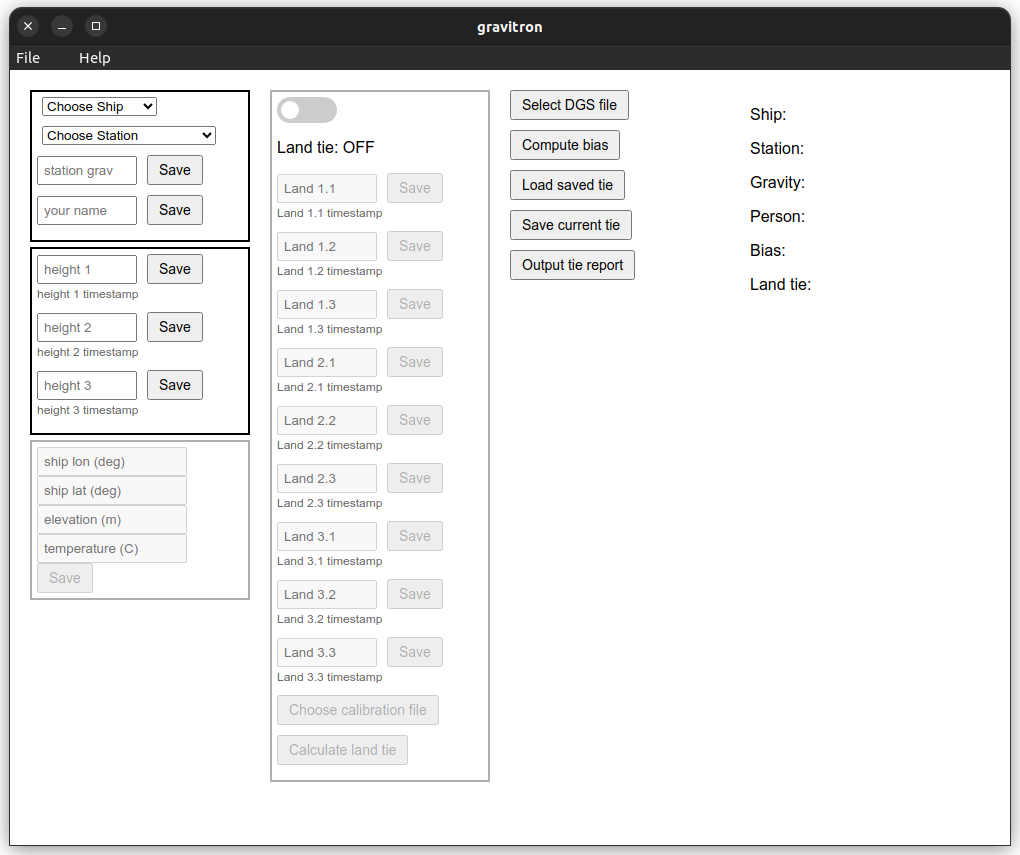
\includegraphics[width=\textwidth]{figs/gravitron_window.png}
\caption{The gravitron window.}
\label{fig:window}
\end{figure}

\subsection{Intro to the gravitron window}

The gravitron window (Figure~\ref{fig:window}) has %%4 loosely defined sections:
%\begin{itemize}
%\item Menus and fields for entering ship/station and (optional) land tie metadata are across the top of the window
%\item Fields for entering land tie count measurements are on the left side of the window
%\item Fields for entering water height measurements are in the center of the window
%\item Buttons for choosing DGS data files, computing bias, saving/loading tie files, and writing out tie reports are on the right side of the window
%\end{itemize}
%
%Buttons and fields that are not active will appear greyed out, and actions taken in gravitron will cause relevant buttons and fields to activate or deactivate. For example, selecting and saving a station will deactivate the station menu and the `Save' button; the `Reset' button will clear selections and reactivate the menu and the save button.
%
\subsection{Steps for taking a tie}
\label{tie-instructions}
%\begin{enumerate}
%\item Start the gravitron program (see Section~\ref{run-gg})
%\item Enter the tie metadata
%    \begin{itemize}
%    \item Select a ship from the dropdown menu and press `Save'
%    \item Select a station from the dropdown menu and press `Save'. If you choose `Other', you will need to enter the station name and the absolute gravity and save both of those. The absolute gravity field will only become active once the station name is saved.
%    \item Enter the name of the tie-taker in the `Personnel' box and save it.
%    \end{itemize}
%\item \textbf{For land ties only:} Click the land tie toggle switch to the `on' position, and enter land meter metadata
%    \begin{itemize}
%    \item Enter the coordinates of the ship (where you will be taking the land tie) in decimal degrees, the elevation in meters, and the temperature in degrees C, and press `save'. All of the fields must be filled in order to save this row of entries; note that it is possible to leave them all blank/unsaved and continue with the land tie if needed.
%    \item Select a land meter from the dropdown and press `Save'. 
%    \item If you choose `Other', you will need to enter the meter name and will also need to supply a calibration file for the meter. Use the `Other cal. file' button to select the calibration file (see Section~\ref{datab}).
%    \end{itemize}
%\item Make pier water height measurements
%    \begin{itemize}
%    \item Measure water height at the pier 3 times, with \textasciitilde 30 minutes elapsing between measurements. Enter each water height (in meters) in the appropriate field in gravitron, and press the corresponding `save' button. 
%    \item[\textbf{Note:}] Pressing `save' tells gravitron that the measurement was taken at the \textit{current time} when the button is pressed. If you aren't saving the water height measurements at the time they are taken, see Section ~\ref{later} for instructions on adjusting timestamps.
%    \end{itemize}
%\item \textbf{For land ties only:} Measure counts with the land meter
%    \begin{itemize}
%    \item Measure counts on the ship three times, recording and saving measurements in gravitron
%    \item Measure counts at the station three times, recording and saving measurements in gravitron
%    \item Again, measure counts on the ship three times, recording and saving measurements in gravitron
%    \item[\textbf{Note:}] Pressing `save' tells gravitron that the measurement was taken at the \textit{current time} when the button is pressed. If you aren't saving the counts measurements at the time they are taken, see Section ~\ref{later} for instructions on adjusting timestamps.
%    \end{itemize}
%\item Use the `Choose DGS file' button to select the file containing `laptop' data for the time period when the water height measurements were taken. You can select multiple files.
%\item \textbf{For land ties only:} Use the `compute land tie' button to compute the land tie value
%\item Use the `compute bias' button to do the bias calculation.
%\item Use the `output report' button to save the gravity tie report
%\item \textbf{Optional, recommended:} Use the `save current tie' button to save the tie to a toml file. This is a file that gravitron can re-read later if any parameters need to be adjusted.
%\end{enumerate}

\subsubsection{What if I made my tie measurements before running gravitron?}
\label{later}
%This is fine, as long as you recorded the (UTC) times at which those measurements were taken.
%
%Follow the steps in Section~\ref{tie-instructions} up to step 4 (or step 5 if taking a land tie). Then, use the `save current tie' button to save the info to a file (NOT a report; see Section~\ref{save-re}). 
%
%Open the file you just saved (with the extension .toml) in a text editor (NOT word; notepad or textedit or gedit should be ok). Edit the timestamps for each of your measurements (water heights and/or land meter counts) to match when the measurements were actually taken. Make sure that the times you put in the file are in UTC and that they match the timestamp formatting in the original toml file. Save the toml file. 
%
%Then, back in gravitron, use the `Load saved tie' button to read the edited toml file. This will load all of your measurements with the correct timestamps. Resume the Section~\ref{tie-instructions} sequence at step 6.

\subsubsection{When do I need to do a land tie?}
Land ties are only necessary when the nearest station with a known gravity measurement is not right next to where the ship is docked -- specifically, if the station is more than 50m away from the ship. Gravity is measured with a calibrated meter on the ship, at the station, and then on the ship again, and those measurements are used to calculate an absolute gravity measurement for the ship's location that is referenced to the established station value.

\subsection{Saving and re-reading ties}
\label{save-re}
%gravitron has two buttons, `save current tie' and `Load saved tie', that enable writing and reading tie information to simple text files separate from tie reports. These files, with the extension .toml, contain key=value pairs for tie information. Things that have not (yet) been entered or calculated in gravitron when a toml file is written will have placeholder values.
%
%You can use this save/load capability to pause and resume working on gravity ties without having to keep the gravitron program open (see also:~\ref{later}). You can also use saved toml files to check that the values gravitron is using for calculations are consistent and correct. 
%
%Note that gravitron doesn't automatically save or read toml files -- it only touches those files when you press the save/load buttons. Any changes made after loading a saved tie are not reflected in the toml file unless you save the tie again.

\subsection{Database files}
\label{datab}
The \texttt{database/} directory that comes with gravitron contains a set of text files with information on UNOLS ships, stations with known gravity measurements, and land meters. There is also a sub-directory \texttt{database/land-cal/} with calibration files for some land meters.

The ship is used in gravitron to determine how DGS files are read. While most UNOLS ships with DGS gravimeters write out `laptop' data files in a common format, there are some exceptions, and we've done our best to accommodate file format differences but we can't plan for ships that we don't know about. Therefore, if you select `Other' for your ship, you will probably not be able to read in a DGS file. You can still record tie measurements and write them out in a toml file, and bias can be calculated later once you or we have figured out how to read the relevant meter file.

The station where a tie is taken should have an associated absolute gravity measurement, which is what the bias calculation is referenced to. If you choose `Other' for your station, or choose a station which does not have a gravity measurement listed in the database, you will have to enter a number for absolute gravity in gravitron in order to compute bias.

%If you are taking a land tie, gravitron will need calibration information for the meter you are using. Calibration files for the meters listed in the gravitron dropdown menu are in the database; if you select `Other' for the meter you will need to supply a calibration file. Meter calibration files are plain text files with three columns: count brackets, corresponding mGal values, and offset factors. Values in each row of the file are separated by a space. A calibrated mGal measurement for a count measurement is calculated by finding the closest count bracket less than the measured counts, and then adding together the corresponding mGal value for that bracket and the offset factor for the bracket multipled by the difference between the bracket and the actual counts.

The database files can also be edited/updated with new information. If there are stations, meters, or ships that should be added, please contact PFPE.

\section{Why do we take gravity ties?}
If you're curious as to why you are being asked to spend 90+ minutes making water height measurements and clicking buttons on your computer, here's a quick explanation of what gravity ties are for.

\subsection{Marine gravimetry in a nutshell}
Gravimetry is the measurement of the strength of a gravitational field. Gravity is typically measured in units of acceleration, such as the Gal (short for galileo) which is defined as 1 cm/s$^2$. Measuring the marine gravity field, either at the sea surface or at depth, can give us information about seafloor bathymetry, the structure of the crust, plate tectonics, and more: once gravity data is corrected for known or assumed effects, the remaining anomalies can be interpreted in terms of local variations in mass/density in the Earth.

Measuring gravity on a large moving platform (like a ship) is difficult \emph{because} the platform is large and moving. Accurately measuring small variations in acceleration due to gravity requires that we be able to compensate and correct for all the other factors that are trying to accelerate the sensor in the gravimeter. Since the gravimeter isn't perfect and gets shaken around at sea, we also need to account for drift in the sensor's measurements over time. Gravity ties, where the ship gravimeter's measurement is referenced to a known gravity measurement in port, enable us to track meter drift by comparing ties taken before and after a cruise. 

\subsection{How DGS meters work}
DGS gravimeters contain AT1M sensors. The AT1M sensor is a scalar gravity/specific force sensor mounted in a 2-axis gyro stable platform that keeps the sensitive axis of the gravity meter aligned with the local gravity vector. The magnitude of the local gravity vector is measured and recorded. Basically, a mass is suspended by a stable metal spring with low temperature sensitivity, and small variations in local gravity are measured based on the electrical current of a Lorentz force actuator which, together with a position detector, keeps the sensing spring at a constant length as the suspended mass experiences changes in the gravitational force and moves in response.

\section{Help!}
\label{helphelp}

\subsection{Troubleshooting}

%\subsubsection{Pre-compiled binaries don't work}
%There are a few reasons why this might happen. First, it's possible that the binary you downloaded was for some reason not set to be executable -- that is, your computer doesn't know that it should be treated as an application. In that case, navigate to the directory containing gravitron in a terminal, use the command\\
%\texttt{chmod +x gravitron} (Linux or Mac OSX) \\
%\texttt{chmod +x gravitron.exe} (Windows) \\
%to make the program executable, and try running it again.
%
%It's also possible that your computer is missing some of the C/GTK libraries that the program expects to be able to find. In that case, try installing gcc and gtk3 by following (part of) the instructions for building from source and see if that helps.
%
%Finally, you may be using a version of your operating system that differs significantly from the version that pre-compiled binary was compiled for. If so, you may need to build the program from source (which, luckily, should be pretty easy to do!) so that it can run on your specific computer.
%
%\subsubsection{Error: could not open the file}
%This means that gravitron can't find the database files which it reads to get lists of ships, stations, and land meters. Make sure that the \texttt{database/} directory is in the directory that contains gravitron, and that you are running gravitron in that directory.
%
%\subsubsection{Error loading CSS file: <broken file>}
%This means that gravitron can't find the \texttt{style.css} file. Make sure that file is in the directory that contains gravitron, and that you are running gravitron in that directory.
%
%\subsubsection{gravitron can't read my DGS data files}
%First, make sure that you are using the `laptop' data files rather than the raw files, as those are what gravitron is designed to read. If that still doesn't work, contact PFPE with a sample of the unreadable file. It may be that gravitron doesn't yet know how to read files from your ship, as there are variations in gravimeter file format between vessels/instruments. Note that you can take and save all of the measurements necessary for a gravity tie and wait until later to compute the bias if there are issues with reading gravimeter files.
%
%\subsubsection{The calculated bias number is really weird}
%There are several possibilities here, but they all boil down to: there's probably some miscommunication between us and the gravitron program. Maybe the timestamps for measurements are incorrect, or the DGS file is not being read properly, or there is some mixup with measurement units. 
%
%You can check some of these possibilities by using the `save current tie' button to write out the info that gravitron has to a toml file, and looking at that file in a text editor. Check to make sure that the timestamps make sense, and that the \texttt{avg\_dgs\_grav} value looks reasonable. Water height measurements should all be in meters, and timestamps must be UTC rather than local time to match what is recorded in the gravimeter files.
%
%Note also that if you try to calculate bias but the DGS data that is loaded into the program does not cover the timespan of your water height measurements, the \texttt{avg\_dgs\_grav} value will default to -99999 so even if the gravity at the pier is calculated correctly the bias will not be.
%
%\subsubsection{My operating system isn't listed in the installation instructions}
%Do you run red hat, fedora, debian, or some other fun linux distro? You should still be able to build gravitron from source, though you will have to figure out the package names for GNU C compilers, GTK3, make, and pkg-config in your system's package manager (if you don't already have those things installed).

\subsubsection{I have some other question that's not answered here}
For specific assistance, contact PFPE.

\subsection{Glossary}
\begin{itemize}
\item \textbf{directory} is another word for `folder' on a computer
\item \textbf{toml} stands for \href{https://toml.io/}{Tom's Obvious Minimal Language}. It's a standard for writing human-readable configuration files similar to INI files.
\item \textbf{gravity} is the force that attracts a body toward any other physical body that has mass.
\end{itemize}

\subsection{Contributing to the code}
Do you have ideas for making gravitron better? Go ahead and \href{https://github.com/hfmark/gravitron/issues}{raise an issue} on the github page or, if you're a savvy C++ programmer, submit a pull request. You can also email PFPE.

\end{document}
